\section{overview}

% \begin{figure*}
%     \centering
%     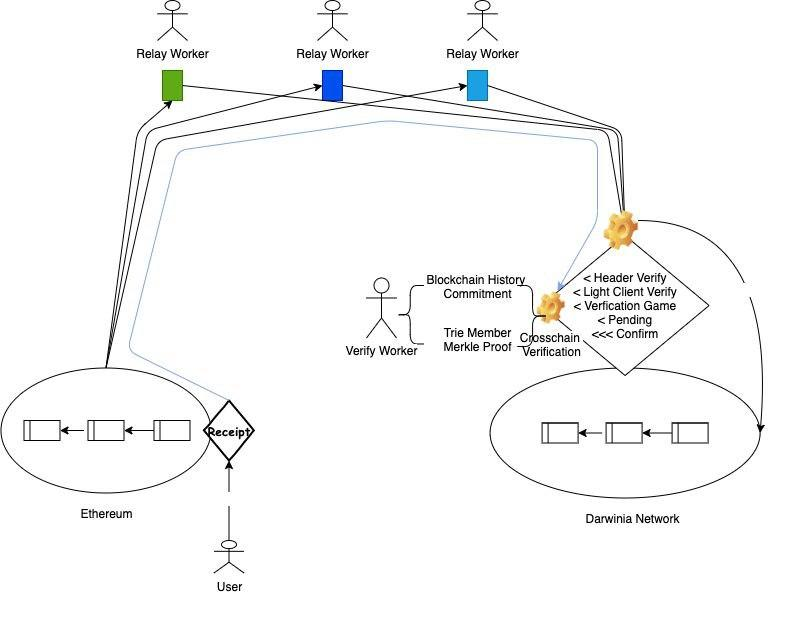
\includegraphics[scale=0.5]{pic/overview.jpg}
%     \caption{Overview}
%     \label{fig:my_label}
% \end{figure*}

For light clients, they need to be able to connect to a complete set of nodes (called certifiers), at least one of which is honest (holding a copy of a valid chain). The light client does not know which one is honest, so Before the light client updates the status, its verification logic needs to be able to identify and filter out the data submitted by those honest nodes. For the off-chain light client, the problem of having at least one honest node can be solved by connecting to the full node, but for the on-chain light client CR, the status update is not made through a network interaction. It is achieved by submitting data to the chain through blockchain transactions through the prover. The cost will be higher, and that's why we need to design reasonable economic incentives to make this process practical.

The outer layer of Darwinia ChainRelay uses verification games as subroutines. The roles in the verification game include a solver who provides a solution for a specific task and a challenger who disagrees with the solver's solution. The final decision role, that is, the referee, can always perform calculations correctly and get results but has extremely limited resources such as computing bandwidth or storage. Darwinia's referee is the entire group of validators, who reach a verdict through systematic consensus.

\subsubsection*{Relay Worker} 

This worker is responsible for verifying, calculating, and submitting the correct block header and its MMR on the chain. Anyone can be a relay worker. The block header and its MMR submitted to the relay on the chain are the solutions. The answer is given by the author. When the solver submits the block header and MMR, he also needs to attach a certain amount of collateral. If a challenger later challenges his results and is found and proved to be cheating by the outer layer, then the system Punishment will be made and its pledge will be confiscated. On the contrary, if there is no challenger to challenge or win in a subsequent verification game, it will prove to be correct and honest, and its pledge will be retrieved and motivated by Relayer Models give rewards.

\subsubsection*{Challenger} 

The challenger is an off-chain role. Anyone can take it. It will monitor each block header, and MMR answers submitted to the Relay on the chain and compare it with the value calculated by itself because the off-chain calculation cost is low ( (No on-chain fees are required), so the challenger can easily calculate the correct value. By comparing the correct value with the submitted value of the solver, if there is a problem, the challenger can determine that he can finally win through the verification game. And make money by getting winning rewards. Qualified challengers are rational and keen monitors. They will seize every opportunity to challenge the solver and win the verification game. If the final verification game finds them false alarms, then the challenger will need to pay the extra cost due to false alarms. Resources, and confiscate the pledge fee attached to its challenge. On the contrary, once it proves that the challenge is successful, it will be rewarded systematically. These rewards are likely to come from pledged items confiscated from the other party's solver.

Base on our assumption, there should be at least one honest Relay Worker. As a result, if this honest Relay Worker finds that the block submitted by other people is different from what he thinks is correct, then he will initiate a verification game as a challenger, and reach a consensus in the end.


\subsubsection*{Judge} 

In our system, Judge is a credible character with fair but expensive computing power. He is a program running on the blockchain. Fig. 2. FLowChart in Section IV shows Judge's behavioral logic.



\subsubsection*{Verification game process} 

The verification game is advanced by a round of fixed duration. The range of each round must be narrowed relative to the last time to allow the verification game to converge to a specific chain. Otherwise, the verification game will continue forever, and it may fail. In Darwinia ChainRelay, the solver and challenger in the verification game need to follow the proof-or-punishment process, because the challenger may not be able to prove that the submitted value of the solver is wrong in only one round, so If you cannot submit a proof, you can narrow the verification calculation by submitting an earlier block header and its MMR. Once entering the verification game, the challenger and the solvers are zero and the opponents of the game. Before the final end, there will be a countdown clock for each round time. If the countdown zero is reached, the opponent does not continue the verification process (proof -or-punishment or result-or-punishment), then the other party wins and the game ends. On the contrary, if the verification game continues, it will converge or partially converge to a range that can be verified on the external chain.


\subsubsection*{Challenge waiting period} Waiting period for the opponent's challenge. After the waiting period, the opponent will give up and the other will win.

